\documentclass[aspectratio=169,11pt]{beamer}
% =====================================================================
%  pds-beamer.tex — Estilo común de las transparencias.
%
%  Uso (desde teoría/Tx/transparencias/):
%     \documentclass[aspectratio=169,11pt]{beamer}
%     % =====================================================================
%  pds-beamer.tex — Estilo común de las transparencias.
%
%  Uso (desde teoría/Tx/transparencias/):
%     \documentclass[aspectratio=169,11pt]{beamer}
%     % =====================================================================
%  pds-beamer.tex — Estilo común de las transparencias.
%
%  Uso (desde teoría/Tx/transparencias/):
%     \documentclass[aspectratio=169,11pt]{beamer}
%     \input{../../comun/pds-beamer}
%     \title{...}  \subtitle{Tema x · ...}
%     \begin{document}
%       \portada
%       ...
%     \end{document}
%  Compilar con:  latexmk -xelatex  (o «make» desde teoría/)
% =====================================================================

\usetheme{Boadilla}
\usecolortheme{orchid}
\usefonttheme{professionalfonts}
\setbeamercovered{transparent}
\setbeamersize{text margin left=0.8cm, text margin right=0.8cm}
\setbeamertemplate{navigation symbols}{}
\setbeamertemplate{itemize item}[square]
\setbeamertemplate{itemize subitem}[circle]
\setbeamertemplate{itemize subsubitem}[triangle]
\setbeamertemplate{enumerate item}[square]
\setbeamertemplate{enumerate subitem}[circle]
\setbeamertemplate{caption}{\raggedright\insertcaption\par}

\input{../../comun/pds-comun.tex}

% Tipografía: Fira Sans + Fira Math (legibles en proyector)
\usepackage{fontspec}
\usepackage{unicode-math}
% Se cargan por nombre de fichero para que funcionen con cualquier
% instalación de TeX Live (o MiKTeX) sin instalar fuentes en el sistema.
\setmainfont{FiraSans}[Extension=.otf, UprightFont=*-Regular, BoldFont=*-SemiBold,
  ItalicFont=*-Italic, BoldItalicFont=*-SemiBoldItalic]
\setsansfont{FiraSans}[Extension=.otf, UprightFont=*-Regular, BoldFont=*-SemiBold,
  ItalicFont=*-Italic, BoldItalicFont=*-SemiBoldItalic]
\setmonofont{FiraMono}[Extension=.otf, UprightFont=*-Regular, BoldFont=*-Medium, AutoFakeSlant=0.15, Scale=0.92]
\setmathfont{FiraMath-Regular.otf}
\setmathfont{latinmodern-math.otf}[range={"229B,"22EE,"22F1}]

% Colores del tema ajustados a la paleta común (más contraste)
\setbeamercolor{structure}{fg=pdsazul}
\setbeamercolor{alerted text}{fg=pdsrojo}
\setbeamercolor{example text}{fg=pdsverde}
\setbeamercolor{block title}{bg=pdsazul, fg=white}
\setbeamercolor{block body}{bg=pdsfondo}
\setbeamercolor{block title alerted}{bg=pdsrojo, fg=white}
\setbeamercolor{block body alerted}{bg=pdsrojo!6}
\setbeamercolor{block title example}{bg=pdsverde, fg=white}
\setbeamercolor{block body example}{bg=pdsverde!6}
\setbeamercolor{frametitle}{fg=pdsazul, bg=white}
\setbeamerfont{frametitle}{size=\large, series=\bfseries}
\setbeamerfont{block title}{size=\normalsize, series=\bfseries}
\setbeamertemplate{blocks}[rounded][shadow=false]

% Logo en la esquina superior derecha de cada transparencia
\pgfdeclareimage[height=0.8cm]{logo}{../../comun/ucm.png}
\addtobeamertemplate{frametitle}{}{%
  \begin{tikzpicture}[remember picture, overlay]
    \node[anchor=north east, inner sep=0pt] at ([xshift=-0.25cm, yshift=-0.2cm]current page.north east) {\pgfuseimage{logo}};
  \end{tikzpicture}}

% Datos de portada
\author[\autorescorto]{\autores}
\institute[UCM]{\footnotesize\departamento\\\universidad}
\date[\curso]{\footnotesize\grado\\\curso}

\newcommand{\portada}{%
  \begin{frame}[plain]
    \begin{center}
      
\includegraphics[height=1.9cm]{../../comun/ucm.png}
    \end{center}
    \vspace{-0.4cm}
    \titlepage
  \end{frame}}

% Índice al empezar cada sección
\AtBeginSection[]{%
  \begin{frame}{Contenido}
    \tableofcontents[currentsection, hideothersubsections]
  \end{frame}}

\renewcommand{\pdscodesize}{\scriptsize}

% Utilidades
% \herramienta{T1-convolucion-continua}: enlace a la página publicada de
% herramientas/html (se abre en el navegador, sin instalar nada).
% \herramientaservidor{server/....py}: app que necesita Python (bokeh serve).
\newcommand{\urlherramientas}{https://ucm-237.github.io/PdS/}
\newcommand{\herramienta}[1]{%
  \par\vfill\hfill{\scriptsize\color{pdsgris}\faIcon\ \href{\urlherramientas#1.html}{Herramienta interactiva: \texttt{#1}}}}
\newcommand{\herramientaservidor}[1]{%
  \par\vfill\hfill{\scriptsize\color{pdsgris}\faIcon\ Herramienta interactiva (con Python): \texttt{herramientas/#1}}}
\newcommand{\faIcon}{\textbf{▶}}
\newcommand{\gris}[1]{{\color{pdsgris}#1}}
\newcommand{\nota}[1]{\par\vspace{2pt}{\footnotesize\color{pdsgris}\textit{#1}}\par}
% Nota sobre una errata de versiones anteriores (solo con \ERRATAS)
\newcommand{\errata}[1]{\iferratas\nota{Errata de versiones anteriores: #1}\fi}
\newcommand{\apuntes}[1]{\nota{Más detalle en los apuntes, #1.}}

% Bloques con nombre en castellano
\newenvironment{definicion}[1][Definición]{\begin{block}{#1}}{\end{block}}
\newenvironment{importante}[1][Importante]{\begin{alertblock}{#1}}{\end{alertblock}}
\newenvironment{ejemplo}[1][Ejemplo]{\begin{exampleblock}{#1}}{\end{exampleblock}}

%     \title{...}  \subtitle{Tema x · ...}
%     \begin{document}
%       \portada
%       ...
%     \end{document}
%  Compilar con:  latexmk -xelatex  (o «make» desde teoría/)
% =====================================================================

\usetheme{Boadilla}
\usecolortheme{orchid}
\usefonttheme{professionalfonts}
\setbeamercovered{transparent}
\setbeamersize{text margin left=0.8cm, text margin right=0.8cm}
\setbeamertemplate{navigation symbols}{}
\setbeamertemplate{itemize item}[square]
\setbeamertemplate{itemize subitem}[circle]
\setbeamertemplate{itemize subsubitem}[triangle]
\setbeamertemplate{enumerate item}[square]
\setbeamertemplate{enumerate subitem}[circle]
\setbeamertemplate{caption}{\raggedright\insertcaption\par}

% =====================================================================
%  pds-comun.tex — Paquetes, colores y estilos de código comunes a
%  transparencias, apuntes y hojas de ejercicios. Compilar con XeLaTeX.
%  No cargar directamente: lo cargan pds-beamer.tex y pds-apuntes.tex.
% =====================================================================

\usepackage{polyglossia}
\setmainlanguage{spanish}
\usepackage{mathtools}
\usepackage{graphicx}
\usepackage{booktabs}
\usepackage{multirow}
\usepackage{array}
\usepackage{xcolor}
\usepackage{tikz}
\usetikzlibrary{positioning,arrows.meta,calc,shapes.geometric,decorations.pathreplacing}
\usepackage{listings}
\usepackage{siunitx}
\sisetup{output-decimal-marker={,}, group-separator={\,}, per-mode=symbol}

% Notas de erratas de versiones anteriores: no se imprimen salvo que se
% defina \ERRATAS antes de cargar el estilo (make ERRATAS=1)
\newif\iferratas
\ifdefined\ERRATAS \erratastrue \fi

% Ruta común (logo y figuras compartidas)
\providecommand{\rutacomun}{../../comun/}
\input{\rutacomun datos.tex}

% ---------------------------------------------------------------------
%  Paleta (la misma que usan las figuras generadas con Python,
%  ver comun/pds_estilo.py)
% ---------------------------------------------------------------------
\definecolor{pdsazul}{HTML}{2B3A8C}
\definecolor{pdsrojo}{HTML}{C0392B}
\definecolor{pdsverde}{HTML}{1E7B4F}
\definecolor{pdsnaranja}{HTML}{D9822B}
\definecolor{pdsgris}{HTML}{5A5A66}
\definecolor{pdsfondo}{HTML}{F3F4FA}
\definecolor{pdscodigo}{HTML}{F7F7F2}

% ---------------------------------------------------------------------
%  Diagramas de bloques (TikZ)
% ---------------------------------------------------------------------
\tikzset{
  bloque/.style={rectangle, rounded corners=2pt, draw=pdsazul!80, fill=pdsfondo,
                 very thick, minimum height=8mm, minimum width=14mm, align=center},
  sumador/.style={circle, draw=pdsazul!80, fill=pdsfondo, thick, inner sep=1.5pt},
  flecha/.style={-{Stealth[length=2.2mm]}, thick, pdsgris},
}

% ---------------------------------------------------------------------
%  Código: Python y Matlab en paralelo
% ---------------------------------------------------------------------
\newcommand{\pdscodesize}{\footnotesize}
\lstdefinestyle{pds}{
  basicstyle=\ttfamily\pdscodesize,
  keywordstyle=\color{pdsazul}\bfseries,
  commentstyle=\color{pdsverde}\itshape,
  stringstyle=\color{pdsrojo},
  numbers=none,
  backgroundcolor=\color{pdscodigo},
  frame=single, rulecolor=\color{pdsgris!40}, framerule=0.4pt,
  xleftmargin=2pt, xrightmargin=2pt, aboveskip=2pt, belowskip=2pt,
  columns=fullflexible, keepspaces=true,
  showstringspaces=false, breaklines=true, tabsize=4,
  upquote=true,
  % Con XeLaTeX, listings desordena los caracteres no ASCII junto a
  % dígitos («2π» sale «π2»): se sustituyen por su versión matemática.
  literate={π}{{$\pi$}}1 {δ}{{$\delta$}}1 {ω}{{$\omega$}}1 {Ω}{{$\Omega$}}1
           {≈}{{$\approx$}}1 {µ}{{$\mu$}}1 {·}{{$\cdot$}}1 {α}{{$\alpha$}}1
           {á}{{á}}1 {é}{{é}}1 {í}{{í}}1 {ó}{{ó}}1 {ú}{{ú}}1 {ñ}{{ñ}}1 {¿}{{¿}}1,
}
\lstdefinestyle{python}{style=pds, language=Python,
  morekeywords={as,True,False,None}}
\lstdefinestyle{matlab}{style=pds, language=Matlab,
  morekeywords={function,end,true,false}}

% \codigo{<ruta sin extensión>} muestra el mismo ejemplo en Python
% y en Matlab, uno al lado del otro. Los ficheros viven en
% ../codigo/python/<nombre>.py y ../codigo/matlab/<nombre>.m y se
% ejecutan en las pruebas (make prueba-codigo).
\newcommand{\rutacodigo}{../codigo/}
\newcommand{\codigoetiqueta}[1]{{\sffamily\scriptsize\bfseries\color{pdsgris}#1}}
\newcommand{\codigo}[2][]{%
  \par\noindent
  \begin{minipage}[t]{0.495\linewidth}
    \codigoetiqueta{Python}\par\vspace{1pt}
    \lstinputlisting[style=python,#1]{\rutacodigo python/#2.py}
  \end{minipage}\hfill
  \begin{minipage}[t]{0.495\linewidth}
    \codigoetiqueta{Matlab}\par\vspace{1pt}
    \lstinputlisting[style=matlab,#1]{\rutacodigo matlab/#2.m}
  \end{minipage}\par}

\input{\rutacomun notacion.tex}


% Tipografía: Fira Sans + Fira Math (legibles en proyector)
\usepackage{fontspec}
\usepackage{unicode-math}
% Se cargan por nombre de fichero para que funcionen con cualquier
% instalación de TeX Live (o MiKTeX) sin instalar fuentes en el sistema.
\setmainfont{FiraSans}[Extension=.otf, UprightFont=*-Regular, BoldFont=*-SemiBold,
  ItalicFont=*-Italic, BoldItalicFont=*-SemiBoldItalic]
\setsansfont{FiraSans}[Extension=.otf, UprightFont=*-Regular, BoldFont=*-SemiBold,
  ItalicFont=*-Italic, BoldItalicFont=*-SemiBoldItalic]
\setmonofont{FiraMono}[Extension=.otf, UprightFont=*-Regular, BoldFont=*-Medium, AutoFakeSlant=0.15, Scale=0.92]
\setmathfont{FiraMath-Regular.otf}
\setmathfont{latinmodern-math.otf}[range={"229B,"22EE,"22F1}]

% Colores del tema ajustados a la paleta común (más contraste)
\setbeamercolor{structure}{fg=pdsazul}
\setbeamercolor{alerted text}{fg=pdsrojo}
\setbeamercolor{example text}{fg=pdsverde}
\setbeamercolor{block title}{bg=pdsazul, fg=white}
\setbeamercolor{block body}{bg=pdsfondo}
\setbeamercolor{block title alerted}{bg=pdsrojo, fg=white}
\setbeamercolor{block body alerted}{bg=pdsrojo!6}
\setbeamercolor{block title example}{bg=pdsverde, fg=white}
\setbeamercolor{block body example}{bg=pdsverde!6}
\setbeamercolor{frametitle}{fg=pdsazul, bg=white}
\setbeamerfont{frametitle}{size=\large, series=\bfseries}
\setbeamerfont{block title}{size=\normalsize, series=\bfseries}
\setbeamertemplate{blocks}[rounded][shadow=false]

% Logo en la esquina superior derecha de cada transparencia
\pgfdeclareimage[height=0.8cm]{logo}{../../comun/ucm.png}
\addtobeamertemplate{frametitle}{}{%
  \begin{tikzpicture}[remember picture, overlay]
    \node[anchor=north east, inner sep=0pt] at ([xshift=-0.25cm, yshift=-0.2cm]current page.north east) {\pgfuseimage{logo}};
  \end{tikzpicture}}

% Datos de portada
\author[\autorescorto]{\autores}
\institute[UCM]{\footnotesize\departamento\\\universidad}
\date[\curso]{\footnotesize\grado\\\curso}

\newcommand{\portada}{%
  \begin{frame}[plain]
    \begin{center}
      
\includegraphics[height=1.9cm]{../../comun/ucm.png}
    \end{center}
    \vspace{-0.4cm}
    \titlepage
  \end{frame}}

% Índice al empezar cada sección
\AtBeginSection[]{%
  \begin{frame}{Contenido}
    \tableofcontents[currentsection, hideothersubsections]
  \end{frame}}

\renewcommand{\pdscodesize}{\scriptsize}

% Utilidades
% \herramienta{T1-convolucion-continua}: enlace a la página publicada de
% herramientas/html (se abre en el navegador, sin instalar nada).
% \herramientaservidor{server/....py}: app que necesita Python (bokeh serve).
\newcommand{\urlherramientas}{https://ucm-237.github.io/PdS/}
\newcommand{\herramienta}[1]{%
  \par\vfill\hfill{\scriptsize\color{pdsgris}\faIcon\ \href{\urlherramientas#1.html}{Herramienta interactiva: \texttt{#1}}}}
\newcommand{\herramientaservidor}[1]{%
  \par\vfill\hfill{\scriptsize\color{pdsgris}\faIcon\ Herramienta interactiva (con Python): \texttt{herramientas/#1}}}
\newcommand{\faIcon}{\textbf{▶}}
\newcommand{\gris}[1]{{\color{pdsgris}#1}}
\newcommand{\nota}[1]{\par\vspace{2pt}{\footnotesize\color{pdsgris}\textit{#1}}\par}
% Nota sobre una errata de versiones anteriores (solo con \ERRATAS)
\newcommand{\errata}[1]{\iferratas\nota{Errata de versiones anteriores: #1}\fi}
\newcommand{\apuntes}[1]{\nota{Más detalle en los apuntes, #1.}}

% Bloques con nombre en castellano
\newenvironment{definicion}[1][Definición]{\begin{block}{#1}}{\end{block}}
\newenvironment{importante}[1][Importante]{\begin{alertblock}{#1}}{\end{alertblock}}
\newenvironment{ejemplo}[1][Ejemplo]{\begin{exampleblock}{#1}}{\end{exampleblock}}

%     \title{...}  \subtitle{Tema x · ...}
%     \begin{document}
%       \portada
%       ...
%     \end{document}
%  Compilar con:  latexmk -xelatex  (o «make» desde teoría/)
% =====================================================================

\usetheme{Boadilla}
\usecolortheme{orchid}
\usefonttheme{professionalfonts}
\setbeamercovered{transparent}
\setbeamersize{text margin left=0.8cm, text margin right=0.8cm}
\setbeamertemplate{navigation symbols}{}
\setbeamertemplate{itemize item}[square]
\setbeamertemplate{itemize subitem}[circle]
\setbeamertemplate{itemize subsubitem}[triangle]
\setbeamertemplate{enumerate item}[square]
\setbeamertemplate{enumerate subitem}[circle]
\setbeamertemplate{caption}{\raggedright\insertcaption\par}

% =====================================================================
%  pds-comun.tex — Paquetes, colores y estilos de código comunes a
%  transparencias, apuntes y hojas de ejercicios. Compilar con XeLaTeX.
%  No cargar directamente: lo cargan pds-beamer.tex y pds-apuntes.tex.
% =====================================================================

\usepackage{polyglossia}
\setmainlanguage{spanish}
\usepackage{mathtools}
\usepackage{graphicx}
\usepackage{booktabs}
\usepackage{multirow}
\usepackage{array}
\usepackage{xcolor}
\usepackage{tikz}
\usetikzlibrary{positioning,arrows.meta,calc,shapes.geometric,decorations.pathreplacing}
\usepackage{listings}
\usepackage{siunitx}
\sisetup{output-decimal-marker={,}, group-separator={\,}, per-mode=symbol}

% Notas de erratas de versiones anteriores: no se imprimen salvo que se
% defina \ERRATAS antes de cargar el estilo (make ERRATAS=1)
\newif\iferratas
\ifdefined\ERRATAS \erratastrue \fi

% Ruta común (logo y figuras compartidas)
\providecommand{\rutacomun}{../../comun/}
\input{\rutacomun datos.tex}

% ---------------------------------------------------------------------
%  Paleta (la misma que usan las figuras generadas con Python,
%  ver comun/pds_estilo.py)
% ---------------------------------------------------------------------
\definecolor{pdsazul}{HTML}{2B3A8C}
\definecolor{pdsrojo}{HTML}{C0392B}
\definecolor{pdsverde}{HTML}{1E7B4F}
\definecolor{pdsnaranja}{HTML}{D9822B}
\definecolor{pdsgris}{HTML}{5A5A66}
\definecolor{pdsfondo}{HTML}{F3F4FA}
\definecolor{pdscodigo}{HTML}{F7F7F2}

% ---------------------------------------------------------------------
%  Diagramas de bloques (TikZ)
% ---------------------------------------------------------------------
\tikzset{
  bloque/.style={rectangle, rounded corners=2pt, draw=pdsazul!80, fill=pdsfondo,
                 very thick, minimum height=8mm, minimum width=14mm, align=center},
  sumador/.style={circle, draw=pdsazul!80, fill=pdsfondo, thick, inner sep=1.5pt},
  flecha/.style={-{Stealth[length=2.2mm]}, thick, pdsgris},
}

% ---------------------------------------------------------------------
%  Código: Python y Matlab en paralelo
% ---------------------------------------------------------------------
\newcommand{\pdscodesize}{\footnotesize}
\lstdefinestyle{pds}{
  basicstyle=\ttfamily\pdscodesize,
  keywordstyle=\color{pdsazul}\bfseries,
  commentstyle=\color{pdsverde}\itshape,
  stringstyle=\color{pdsrojo},
  numbers=none,
  backgroundcolor=\color{pdscodigo},
  frame=single, rulecolor=\color{pdsgris!40}, framerule=0.4pt,
  xleftmargin=2pt, xrightmargin=2pt, aboveskip=2pt, belowskip=2pt,
  columns=fullflexible, keepspaces=true,
  showstringspaces=false, breaklines=true, tabsize=4,
  upquote=true,
  % Con XeLaTeX, listings desordena los caracteres no ASCII junto a
  % dígitos («2π» sale «π2»): se sustituyen por su versión matemática.
  literate={π}{{$\pi$}}1 {δ}{{$\delta$}}1 {ω}{{$\omega$}}1 {Ω}{{$\Omega$}}1
           {≈}{{$\approx$}}1 {µ}{{$\mu$}}1 {·}{{$\cdot$}}1 {α}{{$\alpha$}}1
           {á}{{á}}1 {é}{{é}}1 {í}{{í}}1 {ó}{{ó}}1 {ú}{{ú}}1 {ñ}{{ñ}}1 {¿}{{¿}}1,
}
\lstdefinestyle{python}{style=pds, language=Python,
  morekeywords={as,True,False,None}}
\lstdefinestyle{matlab}{style=pds, language=Matlab,
  morekeywords={function,end,true,false}}

% \codigo{<ruta sin extensión>} muestra el mismo ejemplo en Python
% y en Matlab, uno al lado del otro. Los ficheros viven en
% ../codigo/python/<nombre>.py y ../codigo/matlab/<nombre>.m y se
% ejecutan en las pruebas (make prueba-codigo).
\newcommand{\rutacodigo}{../codigo/}
\newcommand{\codigoetiqueta}[1]{{\sffamily\scriptsize\bfseries\color{pdsgris}#1}}
\newcommand{\codigo}[2][]{%
  \par\noindent
  \begin{minipage}[t]{0.495\linewidth}
    \codigoetiqueta{Python}\par\vspace{1pt}
    \lstinputlisting[style=python,#1]{\rutacodigo python/#2.py}
  \end{minipage}\hfill
  \begin{minipage}[t]{0.495\linewidth}
    \codigoetiqueta{Matlab}\par\vspace{1pt}
    \lstinputlisting[style=matlab,#1]{\rutacodigo matlab/#2.m}
  \end{minipage}\par}

\input{\rutacomun notacion.tex}


% Tipografía: Fira Sans + Fira Math (legibles en proyector)
\usepackage{fontspec}
\usepackage{unicode-math}
% Se cargan por nombre de fichero para que funcionen con cualquier
% instalación de TeX Live (o MiKTeX) sin instalar fuentes en el sistema.
\setmainfont{FiraSans}[Extension=.otf, UprightFont=*-Regular, BoldFont=*-SemiBold,
  ItalicFont=*-Italic, BoldItalicFont=*-SemiBoldItalic]
\setsansfont{FiraSans}[Extension=.otf, UprightFont=*-Regular, BoldFont=*-SemiBold,
  ItalicFont=*-Italic, BoldItalicFont=*-SemiBoldItalic]
\setmonofont{FiraMono}[Extension=.otf, UprightFont=*-Regular, BoldFont=*-Medium, AutoFakeSlant=0.15, Scale=0.92]
\setmathfont{FiraMath-Regular.otf}
\setmathfont{latinmodern-math.otf}[range={"229B,"22EE,"22F1}]

% Colores del tema ajustados a la paleta común (más contraste)
\setbeamercolor{structure}{fg=pdsazul}
\setbeamercolor{alerted text}{fg=pdsrojo}
\setbeamercolor{example text}{fg=pdsverde}
\setbeamercolor{block title}{bg=pdsazul, fg=white}
\setbeamercolor{block body}{bg=pdsfondo}
\setbeamercolor{block title alerted}{bg=pdsrojo, fg=white}
\setbeamercolor{block body alerted}{bg=pdsrojo!6}
\setbeamercolor{block title example}{bg=pdsverde, fg=white}
\setbeamercolor{block body example}{bg=pdsverde!6}
\setbeamercolor{frametitle}{fg=pdsazul, bg=white}
\setbeamerfont{frametitle}{size=\large, series=\bfseries}
\setbeamerfont{block title}{size=\normalsize, series=\bfseries}
\setbeamertemplate{blocks}[rounded][shadow=false]

% Logo en la esquina superior derecha de cada transparencia
\pgfdeclareimage[height=0.8cm]{logo}{../../comun/ucm.png}
\addtobeamertemplate{frametitle}{}{%
  \begin{tikzpicture}[remember picture, overlay]
    \node[anchor=north east, inner sep=0pt] at ([xshift=-0.25cm, yshift=-0.2cm]current page.north east) {\pgfuseimage{logo}};
  \end{tikzpicture}}

% Datos de portada
\author[\autorescorto]{\autores}
\institute[UCM]{\footnotesize\departamento\\\universidad}
\date[\curso]{\footnotesize\grado\\\curso}

\newcommand{\portada}{%
  \begin{frame}[plain]
    \begin{center}
      
\includegraphics[height=1.9cm]{../../comun/ucm.png}
    \end{center}
    \vspace{-0.4cm}
    \titlepage
  \end{frame}}

% Índice al empezar cada sección
\AtBeginSection[]{%
  \begin{frame}{Contenido}
    \tableofcontents[currentsection, hideothersubsections]
  \end{frame}}

\renewcommand{\pdscodesize}{\scriptsize}

% Utilidades
% \herramienta{T1-convolucion-continua}: enlace a la página publicada de
% herramientas/html (se abre en el navegador, sin instalar nada).
% \herramientaservidor{server/....py}: app que necesita Python (bokeh serve).
\newcommand{\urlherramientas}{https://ucm-237.github.io/PdS/}
\newcommand{\herramienta}[1]{%
  \par\vfill\hfill{\scriptsize\color{pdsgris}\faIcon\ \href{\urlherramientas#1.html}{Herramienta interactiva: \texttt{#1}}}}
\newcommand{\herramientaservidor}[1]{%
  \par\vfill\hfill{\scriptsize\color{pdsgris}\faIcon\ Herramienta interactiva (con Python): \texttt{herramientas/#1}}}
\newcommand{\faIcon}{\textbf{▶}}
\newcommand{\gris}[1]{{\color{pdsgris}#1}}
\newcommand{\nota}[1]{\par\vspace{2pt}{\footnotesize\color{pdsgris}\textit{#1}}\par}
% Nota sobre una errata de versiones anteriores (solo con \ERRATAS)
\newcommand{\errata}[1]{\iferratas\nota{Errata de versiones anteriores: #1}\fi}
\newcommand{\apuntes}[1]{\nota{Más detalle en los apuntes, #1.}}

% Bloques con nombre en castellano
\newenvironment{definicion}[1][Definición]{\begin{block}{#1}}{\end{block}}
\newenvironment{importante}[1][Importante]{\begin{alertblock}{#1}}{\end{alertblock}}
\newenvironment{ejemplo}[1][Ejemplo]{\begin{exampleblock}{#1}}{\end{exampleblock}}

\graphicspath{{../figuras/}}

\title[T1 · Operaciones y transformadas]{Introducción: señales y sistemas}
\subtitle{Tema 1 · Parte 2: operaciones con señales y análisis en frecuencia}

\begin{document}
\portada

% =====================================================================
\section{Operaciones sobre la variable independiente}

\begin{frame}{Transformaciones de la variable independiente}
  Cambiamos el «eje de tiempos» sin alterar los valores de la señal:
  \[
    y(t)=x\big(f(t)\big),\qquad y[n]=x\big[f(n)\big]
  \]
  Para $f$ afín, $f(t)=\alpha t+\beta$, se reducen a tres operaciones básicas:
  \begin{center}
    \renewcommand{\arraystretch}{1.25}
    \begin{tabular}{@{}lll@{}}
      \toprule
      & Continua & Discreta\\\midrule
      \alert{Desplazamiento} & $y(t)=x(t-t_0)$ & $y[n]=x[n-n_0]$, \ $n_0\in\Z$\\
      \alert{Inversión} & $y(t)=x(-t)$ & $y[n]=x[-n]$\\
      \alert{Escalado} & $y(t)=x(\alpha t)$, \ $\alpha>0$ & $y[n]=x[Mn]$ \ (diezmado, $M\in\Z^+$)\\
      & & $y[n]=x[n/L]$ \ (expansión, $L\in\Z^+$)\\\bottomrule
    \end{tabular}
  \end{center}
  \begin{itemize}\small
    \item Pueden cambiar la forma de la señal y, en discreto, \alert{perder muestras} (diezmado) o necesitar muestras que no existen (expansión).
  \end{itemize}
\end{frame}

\begin{frame}{Desplazamiento e inversión}
  \begin{columns}[c]
    \begin{column}{0.44\textwidth}
      \begin{itemize}
        \item $x(t-t_0)$: \alert{retardo} si $t_0>0$ (la señal se desplaza a la derecha) y \alert{adelanto} si $t_0<0$.
        \item $x(-t)$: reflejo respecto a $t=0$.
        \item En discreto, $n_0$ debe ser entero.
      \end{itemize}
      \begin{importante}[Cuidado con el signo]
        $x(t-2)$ vale en $t=2$ lo que $x$ valía en $t=0$: está \emph{retrasada} 2 unidades.
      \end{importante}
    \end{column}
    \begin{column}{0.54\textwidth}
      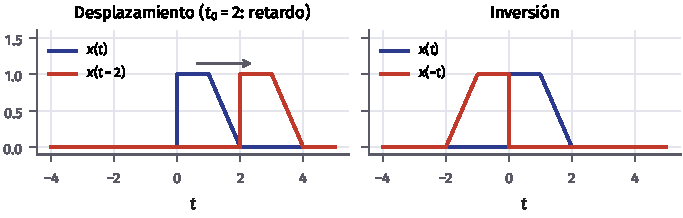
\includegraphics[width=\linewidth]{desplazamiento_inversion}
    \end{column}
  \end{columns}
\end{frame}

\begin{frame}{Escalado temporal}
  \begin{columns}[c]
    \begin{column}{0.5\textwidth}
      \alert{Continuo}: $y(t)=x(\alpha t)$
      \begin{itemize}\small
        \item $\alpha>1$: compresión (la señal «va más rápido»).
        \item $0<\alpha<1$: expansión.
        \item Es reversible: $x(t)=y(t/\alpha)$.
      \end{itemize}
      \medskip
      \alert{Discreto}
      \begin{itemize}\small
        \item \alert{Diezmado}: $y[n]=x[Mn]$, $M\in\Z^+$. Se queda con una de cada $M$ muestras: \alert{se pierde información}.
        \item \alert{Expansión}: $y[n]=x[n/L]$ si $n$ es múltiplo de $L$, y $0$ en otro caso. Las muestras intermedias se rellenan después (interpolación, Tema 2).
      \end{itemize}
    \end{column}
    \begin{column}{0.48\textwidth}
      \centering
      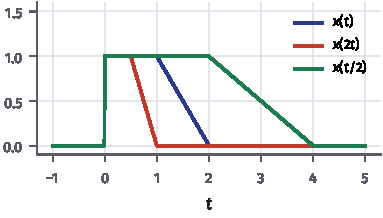
\includegraphics[width=0.75\linewidth]{escalado_continuo}\\[2mm]
      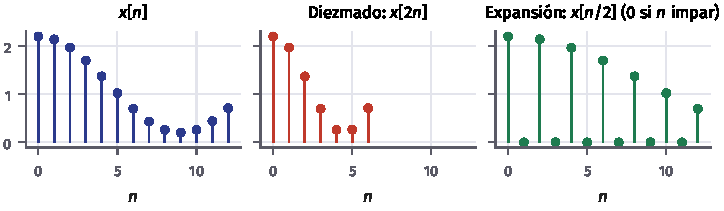
\includegraphics[width=\linewidth]{diezmado_interpolacion}
    \end{column}
  \end{columns}
\end{frame}

\begin{frame}{Transformaciones combinadas: $y(t)=x(\alpha t+\beta)$}
  \begin{block}{Procedimiento seguro: primero desplazar, después escalar}
    \begin{enumerate}
      \item $v(t)=x(t+\beta)$ \quad(desplazamiento)
      \item $y(t)=v(\alpha t)=x(\alpha t+\beta)$ \quad(escalado e inversión si $\alpha<0$)
    \end{enumerate}
  \end{block}
  \begin{center}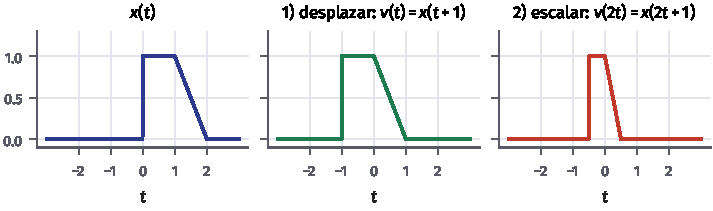
\includegraphics[width=0.7\linewidth]{transformacion_combinada}\end{center}
  \begin{itemize}\small
    \item Comprobación rápida con un punto: el valor que $x$ tenía en $t=0$ aparece en $y$ cuando $2t+1=0$, es decir, en $t=-\tfrac12$.
    \item Hacerlo al revés exige desplazar $\beta/\alpha$: $x(\alpha t+\beta)=x\big(\alpha(t+\beta/\alpha)\big)$.
  \end{itemize}
\end{frame}

% =====================================================================
\section{Operaciones sobre la amplitud}

\begin{frame}{Operaciones básicas con señales}
  \begin{columns}[T]
    \begin{column}{0.5\textwidth}
      \alert{Punto a punto} (continuas y discretas)
      \begin{itemize}\small
        \item Suma: $y=x_1+x_2$
        \item Producto: $y=x_1\cdot x_2$ (modulación, enventanado)
        \item Escalado de amplitud: $y=A\,x$
        \item Cociente: $y=x_1/x_2$ donde $x_2\neq0$
      \end{itemize}
      \medskip
      \alert{Continuas}
      \begin{itemize}\small
        \item Derivada: $y(t)=\dv{x(t)}{t}$
        \item Integral: $y(t)=\displaystyle\int_{-\infty}^{t}x(\tau)\dd\tau$
      \end{itemize}
    \end{column}
    \begin{column}{0.48\textwidth}
      \alert{Discretas}
      \begin{itemize}\small
        \item Diferencia (primera): $y[n]=x[n]-x[n-1]$
        \item Acumulación: $y[n]=\displaystyle\sum_{k=-\infty}^{n}x[k]$
      \end{itemize}
      \begin{block}{Analogía}
        \small
        La diferencia es la versión discreta de la derivada y la acumulación, la de la integral. Por ejemplo,
        $u[n]-u[n-1]=\delta[n]$ y $\sum_{k\le n}\delta[k]=u[n]$, igual que $u'(t)=\delta(t)$.
      \end{block}
    \end{column}
  \end{columns}
\end{frame}

% =====================================================================
\section{Convolución}

\begin{frame}{Convolución}
  \begin{definicion}[Convolución]
    \[
      (x\conv h)(t)=\int_{-\infty}^{\infty}x(\tau)\,h(t-\tau)\dd\tau,
      \qquad
      (x\conv h)[n]=\sum_{k=-\infty}^{\infty}x[k]\,h[n-k]
    \]
  \end{definicion}
  \begin{columns}[T]
    \begin{column}{0.48\textwidth}
      \alert{Procedimiento gráfico} (para cada $t$):
      \begin{enumerate}\small
        \item \alert{Reflejar}: $h(\tau)\to h(-\tau)$
        \item \alert{Desplazar}: $h(-\tau)\to h(t-\tau)$
        \item \alert{Multiplicar}: $x(\tau)\,h(t-\tau)$
        \item \alert{Integrar} (o sumar) en $\tau$
      \end{enumerate}
    \end{column}
    \begin{column}{0.5\textwidth}
      \alert{Propiedades}
      \begin{itemize}\small
        \item Conmutativa: $x\conv h=h\conv x$
        \item Asociativa: $(x\conv h_1)\conv h_2=x\conv(h_1\conv h_2)$
        \item Distributiva: $x\conv(h_1+h_2)=x\conv h_1+x\conv h_2$
        \item Elemento neutro: $x\conv\delta=x$
        \item Desplazamiento: $x(t)\conv\delta(t-t_0)=x(t-t_0)$
        \item Escalón: $(x\conv u)(t)=\int_{-\infty}^{t}x(\tau)\dd\tau$
      \end{itemize}
    \end{column}
  \end{columns}
\end{frame}

\begin{frame}{Convolución continua: ejemplo}
  $x(t)=u(t)-u(t-1)$ (pulso en $[0,1]$) y $h(t)=\e^{-t}u(t)$:
  \begin{center}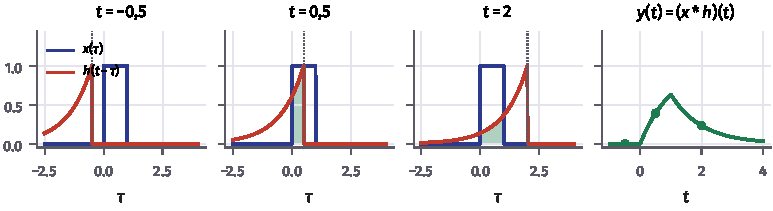
\includegraphics[width=0.8\linewidth]{convolucion_pasos}\end{center}
  \vspace{-3mm}
  \[
    y(t)=\begin{cases}
      0 & t<0 \quad\text{(no se solapan)}\\[1mm]
      \displaystyle\int_0^t\e^{-(t-\tau)}\dd\tau=1-\e^{-t} & 0\le t\le1 \quad\text{(solape parcial)}\\[2mm]
      \displaystyle\int_0^1\e^{-(t-\tau)}\dd\tau=(\e-1)\,\e^{-t} & t>1 \quad\text{(pulso completo)}
    \end{cases}
  \]
  \herramienta{html/T1\_Convolucion continua.html}
\end{frame}

\begin{frame}{Convolución discreta: ejemplo}
  \begin{columns}[c]
    \begin{column}{0.52\textwidth}
      $x[n]=\{\underline{1},2,1\}$, \ $h[n]=\{\underline{1},1,1,1\}$ \ \gris{(subrayado: $n=0$)}
      \medskip

      {\small
      \begin{tabular}{@{}c|cccccc@{}}
        $n$ & 0 & 1 & 2 & 3 & 4 & 5\\\hline
        $x[0]h[n]$ & 1 & 1 & 1 & 1 & & \\
        $x[1]h[n-1]$ & & 2 & 2 & 2 & 2 & \\
        $x[2]h[n-2]$ & & & 1 & 1 & 1 & 1\\\hline
        $y[n]$ & \alert{1} & \alert{3} & \alert{4} & \alert{4} & \alert{3} & \alert{1}
      \end{tabular}}
      \medskip

      {\small Si $x$ tiene $N_x$ muestras y $h$ tiene $N_h$, la convolución tiene $N_x+N_h-1$. Si empiezan en $n_x$ y $n_h$, el resultado empieza en $n_x+n_h$.}
    \end{column}
    \begin{column}{0.46\textwidth}
      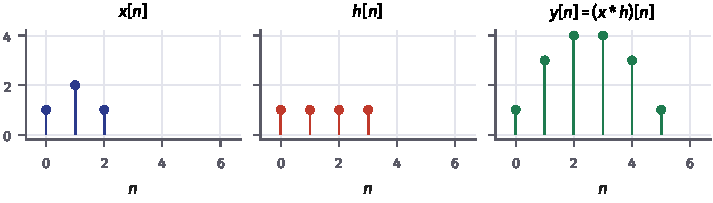
\includegraphics[width=\linewidth]{convolucion_discreta}
    \end{column}
  \end{columns}
\end{frame}

\begin{frame}{En código: convolución discreta}
  \codigo{convolucion}
  \nota{\texttt{np.convolve} y \texttt{conv} no saben dónde empieza cada señal: el índice inicial del resultado es la suma de los índices iniciales.}
  \herramienta{html/T1\_Convolucion discreta.html}
\end{frame}

% =====================================================================
\section{Representación en frecuencia}

\begin{frame}{Idea: descomponer en exponenciales complejas}
  \begin{itemize}
    \item Las exponenciales complejas $\e^{j\Omega t}$ y $\e^{j\omega n}$ son \alert{autofunciones} de los sistemas LTI: salen del sistema multiplicadas por un número complejo (Parte 3).
    \item Si escribimos una señal como suma (o integral) de exponenciales, conocer la respuesta a cada exponencial basta para conocer la respuesta a la señal.
  \end{itemize}
  \begin{center}
    \renewcommand{\arraystretch}{1.3}
    \begin{tabular}{@{}lll@{}}
      \toprule
      & Tiempo continuo & Tiempo discreto\\\midrule
      Periódica & Serie de Fourier: $c_k$ & Serie de Fourier discreta (DFS): $c_k$\\
      Aperiódica & Transformada (CTFT): $\Xc$ & Transformada (DTFT): $\Xd$\\\bottomrule
    \end{tabular}
  \end{center}
  \nota{Periodicidad en un dominio $\leftrightarrow$ espectro discreto (líneas) en el otro. Tiempo discreto $\leftrightarrow$ espectro periódico.}
\end{frame}

\begin{frame}{Serie de Fourier de señales continuas periódicas}
  $x(t)=x(t+T_0)$, \quad $\Omega_0=2\pi/T_0$
  \begin{columns}[T]
    \begin{column}{0.5\textwidth}
      \begin{block}{Forma exponencial}
        Síntesis: \ $x(t)=\displaystyle\sum_{k=-\infty}^{\infty}c_k\,\e^{jk\Omega_0t}$\\[2mm]
        Análisis: \ $c_k=\displaystyle\frac{1}{T_0}\int_{T_0}x(t)\,\e^{-jk\Omega_0t}\dd t$
      \end{block}
    \end{column}
    \begin{column}{0.48\textwidth}
      \begin{block}{Forma trigonométrica ($x$ real)}
        $x(t)=\dfrac{a_0}{2}+\displaystyle\sum_{k=1}^{\infty}\big(a_k\cos(k\Omega_0t)+b_k\sin(k\Omega_0t)\big)$\\[2mm]
        $a_k=\dfrac{2}{T_0}\displaystyle\int_{T_0}x(t)\cos(k\Omega_0t)\dd t$, \quad $b_k=\dfrac{2}{T_0}\displaystyle\int_{T_0}x(t)\sin(k\Omega_0t)\dd t$
      \end{block}
    \end{column}
  \end{columns}
  \begin{itemize}\small
    \item Relación: $c_k=\tfrac12(a_k-jb_k)$ y, si $x$ es real, $c_{-k}=c_k^*$.
    \item $c_0$ es el valor medio. $\abs{c_k}$ y $\arg c_k$ forman el espectro de líneas.
    \item Parseval: $P_x=\dfrac{1}{T_0}\displaystyle\int_{T_0}\abs{x(t)}^2\dd t=\sum_k\abs{c_k}^2$.
  \end{itemize}
\end{frame}

\begin{frame}{Ejemplo: onda cuadrada}
  Onda cuadrada par de amplitud $\pm1$ y ciclo de trabajo del 50\,\%:
  \[
    c_0=0,\qquad c_k=\frac{\sin(\pi k/2)}{\pi k/2}=\sinc(k/2)\ \ (k\neq0)
  \]
  \[
    x(t)=\frac{4}{\pi}\Big(\cos\Omega_0t-\tfrac13\cos3\Omega_0t+\tfrac15\cos5\Omega_0t-\cdots\Big)
  \]
  \vspace{-3mm}
  \begin{center}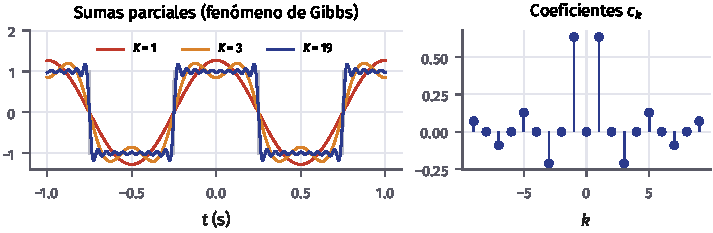
\includegraphics[width=0.72\linewidth]{serie_fourier_cuadrada}\end{center}
  \vspace{-2mm}
  {\small Solo armónicos impares, con amplitud que decae como $1/k$. Cerca de las discontinuidades la suma parcial sobrepasa el salto en torno a un 9\,\% aunque $K$ crezca (\alert{fenómeno de Gibbs}).}
\end{frame}

\begin{frame}{En código: suma parcial de la serie de Fourier}
  \codigo{serie_fourier}
  \nota{Prueba con $K=1,3,19,99$ y observa que el pico de Gibbs no desaparece: solo se estrecha.}
\end{frame}

\begin{frame}{Serie de Fourier discreta (DFS): $x[n]=x[n+N]$}
  \small
  \begin{block}{Forma exponencial: solo hay $N$ armónicos distintos}
    Síntesis: \ $x[n]=\displaystyle\sum_{k=0}^{N-1}c_k\,\e^{j\frac{2\pi}{N}kn}$
    \qquad
    Análisis: \ $c_k=\displaystyle\frac{1}{N}\sum_{n=0}^{N-1}x[n]\,\e^{-j\frac{2\pi}{N}kn}$,
    \quad $c_{k+N}=c_k$
  \end{block}
  \begin{block}{Forma trigonométrica ($x$ real)}
    $x[n]=\dfrac{a_0}{2}+\displaystyle\sum_{k=1}^{L}\Big(a_k\cos\big(\tfrac{2\pi}{N}kn\big)+b_k\sin\big(\tfrac{2\pi}{N}kn\big)\Big)\;\Big[+\tfrac{a_{N/2}}{2}(-1)^n\Big]$\\[2mm]
    $a_k=\dfrac{2}{N}\displaystyle\sum_{n=0}^{N-1}x[n]\cos\big(\tfrac{2\pi}{N}kn\big)$, \quad
    $b_k=\dfrac{2}{N}\displaystyle\sum_{n=0}^{N-1}x[n]\sin\big(\tfrac{2\pi}{N}kn\big)$\\[1mm]
    {\small $L=(N-1)/2$ si $N$ es impar; $L=N/2-1$ más el término entre corchetes si $N$ es par.}
  \end{block}
  {\footnotesize\color{pdsgris}La DFT de un periodo es $X[k]=N c_k$ (Tema 3).}
\end{frame}

\begin{frame}{Transformada de Fourier en tiempo continuo (CTFT)}
  \begin{block}{Definición}
    \[
      \Xc=\int_{-\infty}^{\infty}x(t)\,\e^{-j\Omega t}\dd t,
      \qquad
      x(t)=\frac{1}{2\pi}\int_{-\infty}^{\infty}\Xc\,\e^{j\Omega t}\dd\Omega
    \]
  \end{block}
  \begin{itemize}\small
    \item Es el límite de la serie de Fourier cuando $T_0\to\infty$: las líneas $c_k$ se juntan y el sumatorio pasa a ser una integral.
    \item Existe si $x$ es absolutamente integrable ($\int\abs{x}<\infty$); con deltas se extiende a señales de potencia (sinusoides, escalón).
    \item Si $x$ es real, $X(-j\Omega)=X^*(j\Omega)$: módulo par y fase impar.
  \end{itemize}
\end{frame}

\begin{frame}{CTFT: pares básicos}
  \begin{columns}[c]
    \begin{column}{0.5\textwidth}
      \small
      \begin{tabular}{@{}ll@{}}
        \toprule
        $x(t)$ & $\Xc$\\\midrule
        $\delta(t)$ & $1$\\
        $1$ & $2\pi\,\delta(\Omega)$\\
        $\e^{-at}u(t)$, $a>0$ & $\dfrac{1}{a+j\Omega}$\\
        $\rect(t/T)$ & $T\sinc\!\big(\tfrac{\Omega T}{2\pi}\big)$\\
        $\cos(\Omega_0t)$ & $\pi[\delta(\Omega-\Omega_0)+\delta(\Omega+\Omega_0)]$\\\bottomrule
      \end{tabular}
    \end{column}
    \begin{column}{0.48\textwidth}
      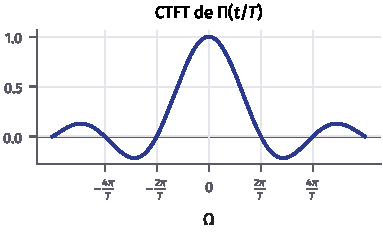
\includegraphics[width=\linewidth]{espectro_ctft_pulso}
    \end{column}
  \end{columns}
\end{frame}

\begin{frame}{Transformada de Fourier en tiempo discreto (DTFT)}
  \begin{block}{Definición}
    \[
      \Xd=\sum_{n=-\infty}^{\infty}x[n]\,\e^{-j\omega n},
      \qquad
      x[n]=\frac{1}{2\pi}\int_{2\pi}\Xd\,\e^{j\omega n}\dd\omega
    \]
  \end{block}
  \begin{itemize}\small
    \item \alert{Periódica en $\omega$ con periodo $2\pi$} (consecuencia de la parte 1). Basta $[-\pi,\pi)$ o $[0,2\pi)$.
    \item Existe si $\sum\abs{x[n]}<\infty$. Se evalúa con \texttt{freqz}.
  \end{itemize}
\end{frame}

\begin{frame}{DTFT: pares básicos}
  \begin{columns}[c]
    \begin{column}{0.52\textwidth}
      \small
      \begin{tabular}{@{}ll@{}}
        \toprule
        $x[n]$ & $\Xd$\\\midrule
        $\delta[n]$ & $1$\\
        $\delta[n-n_0]$ & $\e^{-j\omega n_0}$\\
        $a^n u[n]$, $\abs{a}<1$ & $\dfrac{1}{1-a\e^{-j\omega}}$\\
        $u[n]-u[n-L]$ & $\e^{-j\omega\frac{L-1}{2}}\dfrac{\sin(\omega L/2)}{\sin(\omega/2)}$\\\bottomrule
      \end{tabular}
    \end{column}
    \begin{column}{0.46\textwidth}
      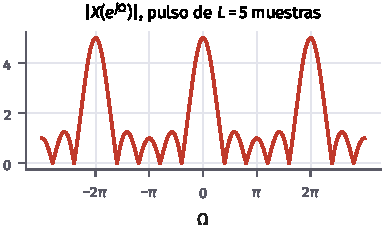
\includegraphics[width=\linewidth]{espectro_dtft_pulso}
    \end{column}
  \end{columns}
\end{frame}

\begin{frame}{En código: DTFT de un pulso}
  \codigo{dtft_pulso}
  \nota{\texttt{freqz} evalúa $X(\e^{j\omega})=\sum_n x[n]\e^{-j\omega n}$ en una rejilla de frecuencias; con \texttt{whole} cubre $[0,2\pi)$ y se ve la periodicidad.}
\end{frame}

\begin{frame}{Propiedades de la transformada de Fourier}
  \small
  \renewcommand{\arraystretch}{1.3}
  \begin{tabular}{@{}lll@{}}
    \toprule
    Propiedad & CTFT & DTFT\\\midrule
    Linealidad & $a x_1+b x_2\parF aX_1+bX_2$ & ídem\\
    Desplazamiento & $x(t-t_0)\parF\e^{-j\Omega t_0}\Xc$ & $x[n-n_0]\parF\e^{-j\omega n_0}\Xd$\\
    Modulación & $\e^{j\Omega_0t}x(t)\parF X(j(\Omega-\Omega_0))$ & $\e^{j\omega_0n}x[n]\parF X(\e^{j(\omega-\omega_0)})$\\
    Escalado & $x(at)\parF\frac{1}{\abs{a}}X\big(j\tfrac{\Omega}{a}\big)$ & —\\
    Derivada / diferencia & $\dv{x}{t}\parF j\Omega\,\Xc$ & $x[n]-x[n-1]\parF(1-\e^{-j\omega})\Xd$\\
    \alert{Convolución} & $x\conv h\parF\Xc H(j\Omega)$ & $x\conv h\parF\Xd H(\e^{j\omega})$\\
    Producto & $x\,y\parF\frac{1}{2\pi}(X\conv Y)(j\Omega)$ & $x\,y\parF\frac{1}{2\pi}\int_{2\pi}X(\e^{j\theta})Y(\e^{j(\omega-\theta)})\dd\theta$\\
    Parseval & $\int\abs{x}^2\dd t=\frac{1}{2\pi}\int\abs{X}^2\dd\Omega$ & $\sum\abs{x}^2=\frac{1}{2\pi}\int_{2\pi}\abs{X}^2\dd\omega$\\\bottomrule
  \end{tabular}
  \bigskip

  La propiedad de \alert{convolución} es la clave del curso: filtrar es multiplicar espectros.
\end{frame}

% =====================================================================
\section{Transformadas de Laplace y Z}

\begin{frame}{Transformada de Laplace}
  \begin{block}{Definición (bilateral)}
    \[
      X(s)=\Lap\{x(t)\}=\int_{-\infty}^{\infty}x(t)\,\e^{-st}\dd t,\qquad s=\sigma+j\Omega\in\C
    \]
    Converge solo en una \alert{región de convergencia} (ROC), una franja vertical $\sigma_1<\Re\{s\}<\sigma_2$.
  \end{block}
  \begin{columns}[c]
    \begin{column}{0.55\textwidth}
      \begin{ejemplo}[La ROC es parte de la transformada]
        \small
        $\e^{-at}u(t)\parL\dfrac{1}{s+a}$, \ \ $\Re\{s\}>-a$\\[1mm]
        $-\e^{-at}u(-t)\parL\dfrac{1}{s+a}$, \ \ $\Re\{s\}<-a$\\[1mm]
        Misma expresión, señales distintas.
      \end{ejemplo}
    \end{column}
    \begin{column}{0.43\textwidth}
      \centering
      \begin{tikzpicture}[scale=0.55]
        \fill[pdsazul!15] (-1,-2) rectangle (3,2);
        \draw[-{Stealth}] (-3,0) -- (3.2,0) node[right]{\scriptsize $\sigma$};
        \draw[-{Stealth}] (0,-2.2) -- (0,2.3) node[above]{\scriptsize $j\Omega$};
        \draw[dashed, pdsazul] (-1,-2) -- (-1,2);
        \node[pdsrojo] at (-1,0) {$\times$};
        \node[below, font=\scriptsize] at (-1,0) {$-a$};
        \node[font=\scriptsize, pdsazul] at (1.6,1.4) {ROC};
        \node[font=\scriptsize, align=center] at (0,-2.8) {señal causal: ROC a la\\derecha del polo};
      \end{tikzpicture}
    \end{column}
  \end{columns}
\end{frame}

\begin{frame}{Laplace: pares y propiedades}
  \small
  Si la ROC contiene el eje $j\Omega$, la CTFT existe y $\Xc=X(s)\big|_{s=j\Omega}$. La versión \alert{unilateral} ($\int_{0^-}^{\infty}$) coincide con la bilateral para señales causales y permite incluir condiciones iniciales.
  \medskip
  \begin{columns}[T]
    \begin{column}{0.46\textwidth}
      \small
      \renewcommand{\arraystretch}{1.3}
      \begin{tabular}{@{}lll@{}}
        \toprule
        $x(t)$ & $X(s)$ & ROC\\\midrule
        $\delta(t)$ & $1$ & todo $\C$\\
        $u(t)$ & $1/s$ & $\Re\{s\}>0$\\
        $t\,u(t)$ & $1/s^2$ & $\Re\{s\}>0$\\
        $\e^{-at}u(t)$ & $\dfrac{1}{s+a}$ & $\Re\{s\}>-a$\\
        $\cos(\Omega_0t)\,u(t)$ & $\dfrac{s}{s^2+\Omega_0^2}$ & $\Re\{s\}>0$\\
        $\sin(\Omega_0t)\,u(t)$ & $\dfrac{\Omega_0}{s^2+\Omega_0^2}$ & $\Re\{s\}>0$\\\bottomrule
      \end{tabular}
    \end{column}
    \begin{column}{0.52\textwidth}
      \small
      \renewcommand{\arraystretch}{1.3}
      \begin{tabular}{@{}ll@{}}
        \toprule
        Propiedad & \\\midrule
        Linealidad & $a x_1+b x_2\parL aX_1+bX_2$\\
        Desplazamiento & $x(t-t_0)\parL\e^{-st_0}X(s)$\\
        Desplaz. en $s$ & $\e^{s_0t}x(t)\parL X(s-s_0)$\\
        Derivada & $\dv{x}{t}\parL sX(s)$\\
        \quad (unilateral) & $\dv{x}{t}\parL sX(s)-x(0^-)$\\
        Integral & $\int_{-\infty}^{t}x\dd\tau\parL X(s)/s$\\
        \alert{Convolución} & $x\conv h\parL X(s)H(s)$\\\bottomrule
      \end{tabular}
    \end{column}
  \end{columns}
\end{frame}

\begin{frame}{Transformada Z}
  \begin{block}{Definición (bilateral)}
    \[
      X(z)=\Zt\{x[n]\}=\sum_{n=-\infty}^{\infty}x[n]\,z^{-n},\qquad z=r\e^{j\omega}\in\C
    \]
    La ROC es una \alert{corona} $r_1<\abs{z}<r_2$.
  \end{block}
  \begin{columns}[c]
    \begin{column}{0.55\textwidth}
      \begin{ejemplo}[La ROC es parte de la transformada]
        \small
        $a^n u[n]\parZ\dfrac{1}{1-az^{-1}}$, \ \ $\abs{z}>\abs{a}$\\[1mm]
        $-a^n u[-n-1]\parZ\dfrac{1}{1-az^{-1}}$, \ \ $\abs{z}<\abs{a}$
      \end{ejemplo}
    \end{column}
    \begin{column}{0.43\textwidth}
      \centering
      \begin{tikzpicture}[scale=0.62]
        \fill[pdsazul!15] (-2.2,-2.2) rectangle (2.2,2.2);
        \fill[white] (0,0) circle (0.8);
        \draw[-{Stealth}] (-2.4,0) -- (2.5,0) node[right]{\scriptsize Re};
        \draw[-{Stealth}] (0,-2.4) -- (0,2.5) node[above]{\scriptsize Im};
        \draw[dashed, pdsgris] (0,0) circle (1.5);
        \draw[dashed, pdsazul] (0,0) circle (0.8);
        \node[pdsrojo] at (0.8,0) {$\times$};
        \node[below right, font=\scriptsize] at (0.75,0) {$a$};
        \node[font=\scriptsize, pdsgris] at (1.35,1.45) {$\abs{z}=1$};
        \node[font=\scriptsize, pdsazul] at (-1.5,-1.7) {ROC};
      \end{tikzpicture}
    \end{column}
  \end{columns}
\end{frame}

\begin{frame}{Z: pares y propiedades}
  \small
  Si la ROC contiene la circunferencia unidad, la DTFT existe y $\Xd=X(z)\big|_{z=\e^{j\omega}}$. Señales causales: ROC exterior a un círculo. La unilateral ($\sum_{n\ge0}$) incluye condiciones iniciales.
  \medskip
  \begin{columns}[T]
    \begin{column}{0.48\textwidth}
      \footnotesize
      \renewcommand{\arraystretch}{1.3}
      \begin{tabular}{@{}lll@{}}
        \toprule
        $x[n]$ & $X(z)$ & ROC\\\midrule
        $\delta[n]$ & $1$ & todo $\C$\\
        $u[n]$ & $\dfrac{1}{1-z^{-1}}$ & $\abs{z}>1$\\
        $a^nu[n]$ & $\dfrac{1}{1-az^{-1}}$ & $\abs{z}>\abs{a}$\\
        $n\,a^nu[n]$ & $\dfrac{az^{-1}}{(1-az^{-1})^2}$ & $\abs{z}>\abs{a}$\\
        $\cos(\omega_0n)\,u[n]$ & $\dfrac{1-\cos\omega_0\,z^{-1}}{1-2\cos\omega_0\,z^{-1}+z^{-2}}$ & $\abs{z}>1$\\\bottomrule
      \end{tabular}
    \end{column}
    \begin{column}{0.5\textwidth}
      \footnotesize
      \renewcommand{\arraystretch}{1.3}
      \begin{tabular}{@{}ll@{}}
        \toprule
        Propiedad & \\\midrule
        Linealidad & $a x_1+b x_2\parZ aX_1+bX_2$\\
        Desplazamiento & $x[n-n_0]\parZ z^{-n_0}X(z)$\\
        \quad (unilateral) & $x[n-1]\parZ z^{-1}X(z)+x[-1]$\\
        \quad (unilateral) & $x[n+1]\parZ zX(z)-z\,x[0]$\\
        Escalado en $z$ & $a^nx[n]\parZ X(z/a)$\\
        \alert{Convolución} & $x\conv h\parZ X(z)H(z)$\\\bottomrule
      \end{tabular}
    \end{column}
  \end{columns}
\end{frame}

\begin{frame}{Relación entre las transformadas}
  \begin{center}
    \begin{tikzpicture}[node distance=1.1cm and 4.2cm, every node/.style={font=\small}]
      \node[bloque] (L) {Laplace $X(s)$};
      \node[bloque, right=of L] (Z) {Z \ $X(z)$};
      \node[bloque, below=of L] (F) {CTFT $\Xc$};
      \node[bloque, below=of Z] (D) {DTFT $\Xd$};
      \draw[flecha] (L) -- node[left, align=right]{$s=j\Omega$\\\scriptsize(ROC $\ni$ eje $j\Omega$)} (F);
      \draw[flecha] (Z) -- node[right, align=left]{$z=\e^{j\omega}$\\\scriptsize(ROC $\ni$ $\abs{z}=1$)} (D);
      \draw[flecha, dashed] (L) -- node[above]{muestreo $t=nT_s$} node[below]{$z=\e^{sT_s}$} (Z);
      \draw[flecha, dashed] (F) -- node[below]{$\omega=\Omega T_s$} (D);
    \end{tikzpicture}
  \end{center}
  \begin{columns}[T]
    \begin{column}{0.5\textwidth}
      \alert{Laplace y Z}
      \begin{itemize}\small
        \item Resolver ecuaciones diferenciales y en diferencias.
        \item Función de transferencia, polos, ceros y estabilidad de sistemas LTI.
      \end{itemize}
    \end{column}
    \begin{column}{0.5\textwidth}
      \alert{Fourier (CTFT y DTFT)}
      \begin{itemize}\small
        \item Contenido en frecuencia de señales.
        \item Respuesta en frecuencia de sistemas LTI estables.
        \item Respuesta en régimen permanente: $Y=H\cdot X$.
      \end{itemize}
    \end{column}
  \end{columns}
\end{frame}

% =====================================================================
\section*{Resumen}
\begin{frame}{Conceptos importantes}
  \begin{columns}[T]
    \begin{column}{0.5\textwidth}
      \begin{itemize}
        \item Operaciones sobre la variable: desplazamiento, inversión, escalado; diezmado y expansión en discreto.
        \item Para $x(\alpha t+\beta)$: primero desplazar, después escalar.
        \item Operaciones sobre la amplitud; derivada/diferencia e integral/acumulación.
        \item \alert{Convolución}: definición, cálculo gráfico y propiedades.
      \end{itemize}
    \end{column}
    \begin{column}{0.5\textwidth}
      \begin{itemize}
        \item Series de Fourier (continua y discreta) y transformadas CTFT y DTFT.
        \item La DTFT es periódica de periodo $2\pi$.
        \item Laplace y Z bilaterales: \alert{siempre con su ROC}.
        \item Convolución en el tiempo $\leftrightarrow$ producto en frecuencia.
      \end{itemize}
    \end{column}
  \end{columns}
  \bigskip
  \gris{Apuntes del Tema 1, secciones 4–6 · Hoja de ejercicios, ejercicios 5–8.}
\end{frame}

\end{document}
